%%%%%%%%%%%%%%%%%%%%%%%%%%%%%%%%%%%%%%%%
%% MCM/ICM LaTeX Template %%
%% 2021 MCM/ICM           %%
%%%%%%%%%%%%%%%%%%%%%%%%%%%%%%%%%%%%%%%%
\documentclass[12pt]{article}
\usepackage{geometry}
%\usepackage{setspace}


\geometry{left=1in,right=0.75in,top=1in,bottom=1in}
%%%%%%%%%%%%%%%%%%%%%%%%%%%%%%%%%%%%%%%%
% Replace ABCDEF in the next line with your chosen problem
% and replace 1111111 with your Team Control Number
\newcommand{\Problem}{C}
\newcommand{\Team}{2103994}
%%%%%%%%%%%%%%%%%%%%%%%%%%%%%%%%%%%%%%%%

\usepackage{newtxtext}
\usepackage{amsmath,amssymb,amsthm}
\usepackage{newtxmath} % must come after amsXXX
\usepackage{graphicx}
\usepackage{xcolor}
\usepackage{fancyhdr}
\lhead{Team \Team}
\rhead{}
\cfoot{}

\newtheorem{theorem}{Theorem}
\newtheorem{corollary}[theorem]{Corollary}
\newtheorem{lemma}[theorem]{Lemma}
\newtheorem{definition}{Definition}

%%%%%%%%%%%%%%%%%%%%%%%%%%%%%%%%
%================================
\usepackage{enumerate}%\item 需要
\usepackage{tabularx}% \table 
\usepackage{booktabs}% 	\toprule
\usepackage{float}%图片浮动
\usepackage{graphicx}
\usepackage{bm}% reference
\usepackage{indentfirst} 
\setlength{\parindent}{2em} %2em代表首行缩进两个字符
\usepackage{listings}%代码
%================================
\begin{document}
%\graphicspath{{.}}  % Place your graphic files in the same directory as your main document
%\DeclareGraphicsExtensions{.pdf, .jpg, .tif, .png}
\thispagestyle{empty}
\vspace*{-16ex}
\centerline{\begin{tabular}{*3{c}}
	\parbox[t]{0.3\linewidth}{\begin{center}\textbf{Problem Chosen}\\ \Large \textcolor{red}{\Problem}\end{center}}
	& \parbox[t]{0.3\linewidth}{\begin{center}\textbf{2021\\ MCM/ICM\\ Summary Sheet}\end{center}}
	& \parbox[t]{0.3\linewidth}{\begin{center}\textbf{Team Control Number}\\ \Large \textcolor{red}{\Team}\end{center}}	\\
	\hline
\end{tabular}}

%==========================================
\renewcommand{\abstractname}{Summary}

%=====================================
%%%%%%%%%%% Begin Summary %%%%%%%%%%%
% Enter your summary here replacing the (red) text
% Replace the text from here ...

\begin{center}
	\large\textbf{  { Data-Driven Model for Asian Hornet Detection with \\ imbalanced and limited dataset}}
	\end{center}
\begin{abstract}
As Asian Hornet invadeds Washington State, the public voluntarily provide information about the insects they have seen or captured which looked  like the hornet. And to analysis the spread of the hornet and distinguish  the insect, we use \textbf{hypothesis testing theory} to prove that the spread of hornet is random and the pest has been eradicated in Washington States. We also set up\textbf{ multimodal classification model} to classify Asian Hornet through the reports.

The classification model uses the image, video, text and other information a record given and is trained by the labelled samples.

\begin{enumerate}[\bf 1.]
	
	
	\item Firstly, We process the video by \textbf{scene detection}to get \textbf{video keyframes}. And use \textbf{Yolo V5}  to automate \textbf{object box annotation}. We vectorize the text by \textbf{N-grams} coding and code time and position as well.
	
	\item Secondly, we use \textbf{Inception V4} to do hornet image classification and get the probability as a feature and get another feature by \textbf{ridge regression} on text coding result.
	
	\item Finally, we combine all the features with longitude, latitude, date as independent variable to do \textbf{logistic regression} on lable to get the classifier.
	
\end{enumerate}

We note that the sample set is quite imbalance for the amount of positive sample is much smaller than positive sample, so we use \textbf{data augmentation} when deal with images, and use \textbf{focal loss} as loss function to train Inception net. We also enhance sample by using \textbf{over-sampling} algorithm \textbf{ADASNY}.

Also we keep the model to be \textbf{online trainable}, so once a new sample comes, we can adjust the model at once. This is realized by \textbf{ fine-tune} and \textbf{FTRL}.


We also test every part of the model is neccessary and propriate by \textbf{Alation Experiment} and other hypothesis testing methods.

In conclusion, a robust, transferable,  multimodal, online learning model is established to classify the reports. And test the situation of hornet invasion in statistics methods.


\textbf{Keywords}:  Multimodal Classification, Hornet Detection, Imbalanced sample, Online learning

\end{abstract}
% to here
%%%%%%%%%%% End Summary %%%%%%%%%%%

%%%%%%%%%%%%%%%%%%%%%%%%%%%%%%
\clearpage
\pagestyle{fancy}
% Uncomment the next line to generate a Table of Contents
\tableofcontents 
\newpage
\setcounter{page}{1}


%\setlength{\baselineskip}{5pt}


\rhead{Page \thepage\ }
%%%%%%%%%%%%%%%%%%%%%%%%%%%%%%


\section{Introduction}
\subsection{Problem Background}
\subsubsection{Asian Giant Hornet Invading  }
Vespa mandarinia is the largest species of hornet in the world, and the occurrence of the nest was alarming. Additionally, the giant hornet is a predator of European honeybees, invading and destroying their nests. A small number of the hornets are capable of destroying a whole colony of European honeybees in a short time. At the same time, they are voracious predators of other insects that are considered agricultural pests.

In September 2019, a colony of Vespa mandarinia (also known as the Asian giant hornet) was discovered on Vancouver Island in British Columbia, Canada. The nest was quickly destroyed, but the news of the event spread rapidly throughout the area. 

From the first report of Asian giant hornets received, the public has played a critical role in the detection of Asian giant hornets in the Pacific Northwest. Washington State Department of Agriculture(WSDA)  has set up platforms\cite{fb} to collect informations from the  public and set traps to get hornets.  
 
\subsubsection{Asian Giant Hornet  }
\begin{figure}[!htbp]
	\small
	\centering
	\begin{minipage}{8cm}
		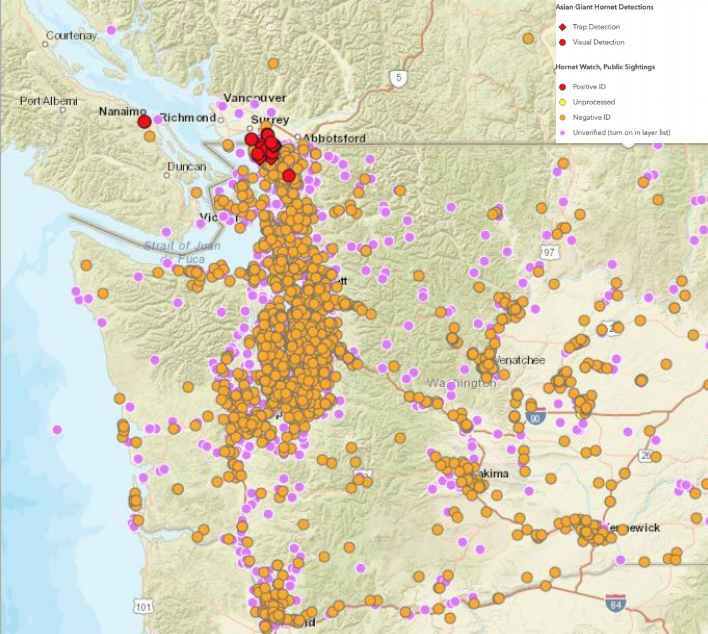
\includegraphics[width=7cm,height=7cm]{./pictures/dist0.png}
		\caption{ Asian Giant Hornet Detections\cite{website}}\label{nt}
	\end{minipage}
	\begin{minipage}{8cm}
		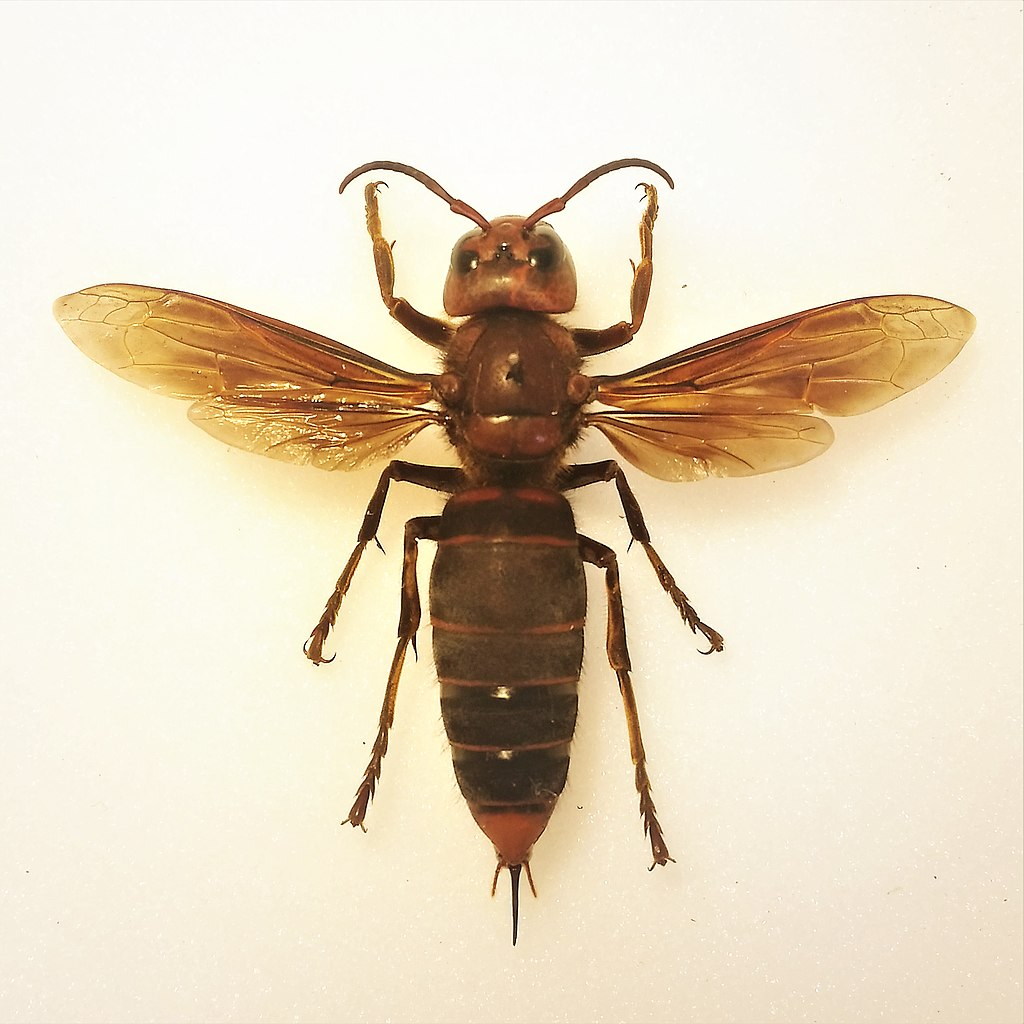
\includegraphics[width=7cm,height=7cm]{./pictures/wikiintro.jpg}
		\caption{\emph{Vespa mandarinia}\cite{wiki}}\label{nt}
	\end{minipage}
	
\end{figure}

\textbf{Name}

Common name:  Asian giant hornet, sparrow wasp, murder hornet

Scientific name: Vespa mandarinia Smith, 1852

\textbf{Range of Activity }

Usually to find food, the Asian giant hornet goes only 0.5 to 1.25 miles (1-2 kilometers) away from the nest (and never more than 5 miles (8 kilometers)) .

\textbf{Life Period}

 Like other social wasps, Asian giant hornets are an annual species that build new nests every year. When winter arrives, the current seasons' nests die out and the only individuals that survive are overwintering queens. When overwintering queens emerge in the spring, they seek out protected areas in the ground to begin building a nests.
\quad\\
 
\textbf{Comparision with Other Species}

While Asian giant hornets do not occur in eastern North America, there are a number of other large wasps that may be confused for them.Here introduce some species alike and there distinctions.
\begin{table}[]
\begin{tabular}{|l|l|l|}
\hline
Species         & Similarity                               & Distinguish                 \\ \hline
Asian Giant Hornet &
  \begin{tabular}[c]{@{}l@{}}around 1.5 inches, yellow head,\\ black belly, live on the ground \\ or lower than 6 feet\end{tabular} &
   \\ \hline
VespaCabro &
  size, shape, color are simlilar &
  \begin{tabular}[c]{@{}l@{}}small differences on face and\\ chest, live higher than 6 feet\end{tabular} \\ \hline
VespulaSquamosa & only the queen may be confused in spring & much smaller in size        \\ \hline
cicada killers  & simliar size                             & no yellow in head and belly \\ \hline
Dolichovespula Maculata &
   &
  \begin{tabular}[c]{@{}l@{}}small size, in the color of\\ black and white, live on the \\ tree or reef\end{tabular} \\ \hline
\end{tabular}
\caption{Comparison of Similar Species}
\label{tab:Similar Species}
\end{table}


\subsection{Our work}
\begin{itemize}
	\item Firstly, we try to predict the spread of hornet, but just find that the spread is not regulated and can be regarded as random walk by examine the independency of report locations.
	\item Secondly, from all the information WSDA recieved, several confirmed sightings of the pest have occurred in neighboring Washington State, as well as a multitude of mistaken sightings. So we construct a model to distinguish whether or not the observed object in one sighting record is Asian Giant Hornet.
	\item Then, we use this model to classify unverified records.
	\item After that, we discuss methods to update the model as new data comes in.
	\item Finally, we use the result to verify that the hornet in Washington State has been readicated.
\end{itemize}


\section{Assumptions}

To simplify our model and eliminate the complexity, we make the following main assumptions in this literature. All assumptions will be re-emphasized once they are used in the construction of our model:
\begin{enumerate}[\bfseries 1.]
	\item The first arrival of Asian Giant Hornet in the United States is the first found in Washington State (time: 2019/9/19; latitude: 49.149394; longitude: -123.943134)
	\item Under the control of authoritied concerned, the distance and time of the spread of hornet are limited.
	\item For unverified, unprocessed and potential sightings, some of their features are similar to the verified ones', so we can build a data-driven model.
\end{enumerate}


\section{Task 1: The Spread of Hornet}

To decide whether the spread of hornets can be predicted based the collected. We introduce the hypothesis test theory in statistics to test whether the time series of the longitude and the latitude is a white noise sequence (random sequence) or not. In \textbf{theory of time series analysis}, the Ljung-Box test is a test designed for judge the randomness of a time series data. It rejects  the null analysis if the data isn’t random. In that case, we can perform some methods of time series analysis for prediction. If it accepts the null analysis, then we can draw the conclusion that this sequence is random and can not be used for prediction.

We divide our process into two steps: 

First, preprocess the data and perform visualization of the data to draw some qualitative conclusion.

Secondly, we perform the Ljung-Box test and draw the Quantitative conclusion.

\subsection{Data Preprocessing}
Firstly we want to know about the basic information of these sighting records.
\begin{table}[H]
	\caption{Basic Information of records}  
	\small
	\begin{center}  
		\begin{tabular}{|m{7cm}<{\centering}|m{7cm}<{\centering}|}  
			\hline  
			Positive number & 14  \\ \hline  
			Negative number& 2096\\ \hline  
			Unverified number &2342 \\  
			\hline 
			Unprocessed & 15 \\  
			\hline  
			Date range &1980   to   2020 \\  
			\hline
		    Latitude range & 45.4886  --   49.5480\\  
			\hline
			Longitude range & -124.6650   --  116.8736\\  
			\hline
		\end{tabular}  
	\end{center}  
\end{table}

According to the table above, we decide to choose process data in these way:
\begin{itemize}
	\item Select positive ID and unverified sample to anlysis. That's because the sample of Positive ID is too small and  random.
	\item Use the average position of each month's sighting site as the center of hornet, and search the tend of the species by the change of center point.
	\item Use the data after March, 2019. For it's when the first confirmed sighting appeared.
\end{itemize}

\begin{figure}[H]
	\centering
	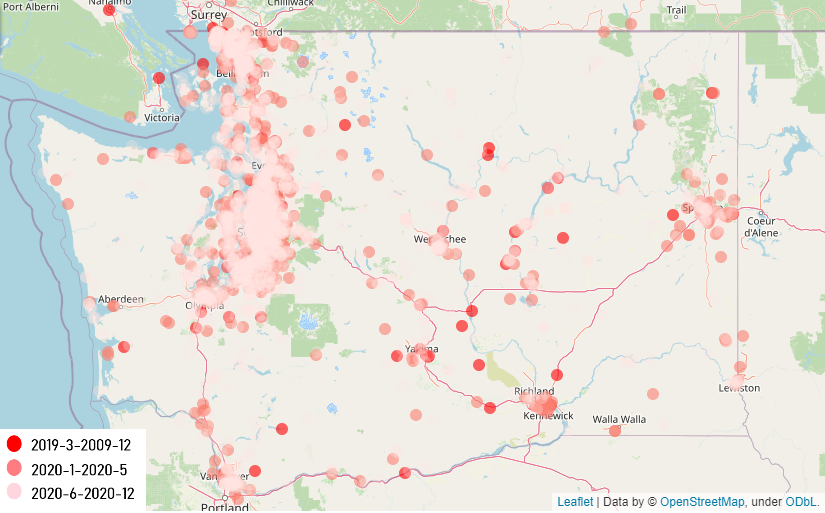
\includegraphics[width=14cm,height=7cm]{./pictures/distribute1.png}
	\caption{sighting sites}
\end{figure}

\begin{figure}[H]
	\small
	\centering
	\begin{minipage}{8cm}
		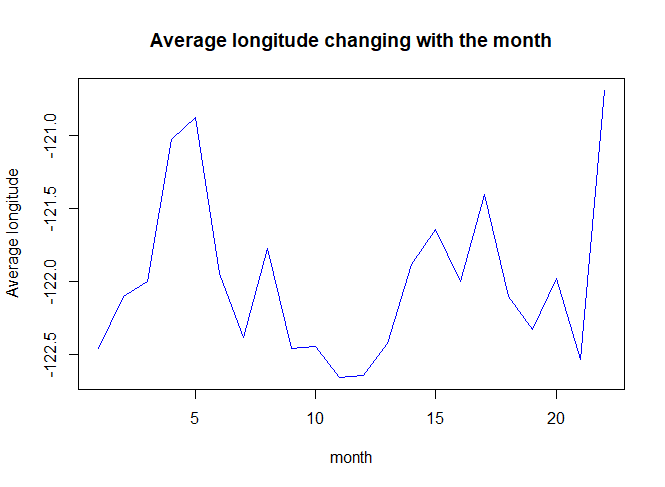
\includegraphics[width=8cm,height=7cm]{./pictures/longtitude.png}
		\label{nt}
	\end{minipage}
	\begin{minipage}{8cm}
		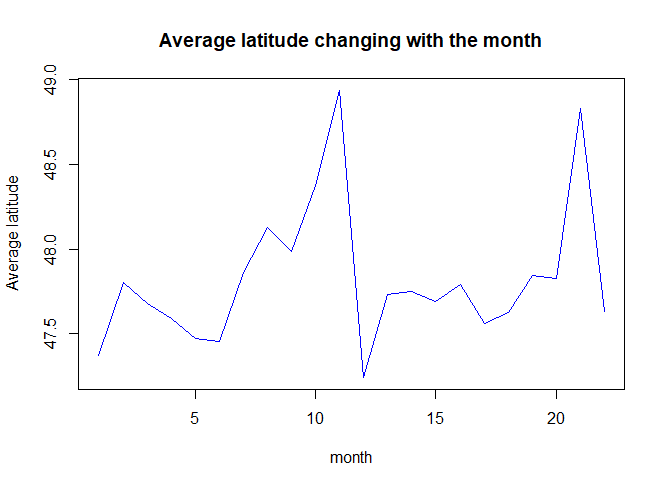
\includegraphics[width=8cm,height=7cm]{./pictures/latitude.png}
		\label{nt}
	\end{minipage}
	\caption{The change of center point}
\end{figure}
From the pictures above, we find out that the movement of hornet is quite random, so we need to use some statistic methods to approve that.

\subsection{Hypothesis Testing}
\subsubsection{Model}
We want to test whether the center points of hornet are independent or the route of the colony has some regulation.So we hypothesis that:
\begin{equation*}
H0:\textbf{These center points are independent }\leftrightarrow H1:\textbf{These center points are not independent}
\end{equation*}

And for it's two dimension data, we test the regulation in longitude and latitude apparently.

As we use $\rho_i$ to represent the k-order lag correlation coefficient of the sample's longtitude. The  hypothesis can be writen as:
\begin{equation*}
H0:\rho_1^2=\rho_2^2=...\rho_h^2=0 \leftrightarrow H1:\exists k,s.t. \rho_k^2\neq 0
\end{equation*}
And choose pivot quantity
\begin{equation}
Q=n(n+1)\sum_{k=1}^h \frac{\rho_k^2}{n-k},\qquad ,h:degree \,of\, randomness
\end{equation}
For $Q\sim \chi^2(h)$, as significance level is $alpha$,the rejection region is $Q> \chi^2_{\alpha-1}(h)$.

In the same way, we test the randomness of the latitude data by using latitude information to calculate $\bar\rho_i\,and\,\bar{Q}$.

\subsubsection{Conclusion}
According to calculating result,neither $Q$ and $\bar{Q}$ doesn't fall in the  the rejection region even in the significance level of 0.5 (P-value are above 0.5 in whatever the randomness is ). \textbf{That means we can't say the spread of hornet can be predicted even the accuracy is 0.5}

\section{Task 2:Classification Model}
\subsection{Model Introduction}
From all the records we get information in quite a lot of forms including \textbf{word, image, video and so on}.
\begin{itemize}
	\item \textbf{Video}: video of the recorded object, including video after capture the insect, surveillance video contains the insect, video of outdoor observation and so on.
	\item \textbf{Image}: image with the recorded insect held on hand, captured by bottle, on a web,in flowers and so on.
	\item \textbf{Word}: notes recorded by the observer; comments replied by the officer。
	\item \textbf{Other information}: longitude and latitude of the sighting site and the date.
	\item \textbf{Label Status}: whether or not the object is Asian Giant Hornet , including unverified.
\end{itemize}

So, we choose \textbf{Multimodal machine learning} to classify the records.
That means we use all the given information to construct the classification model.

\quad \\
Another key porblem of this issue is: the positive sample is too small (14 compared with the negative sample number:2096). So the \textbf{sample imbalance} is great. We use \textbf{sample augmentation, focal loss, oversampling} to deal with this problem.

A more detailed explaination of the model can be seen in the picture below:
\begin{figure}[H]
	\centering
	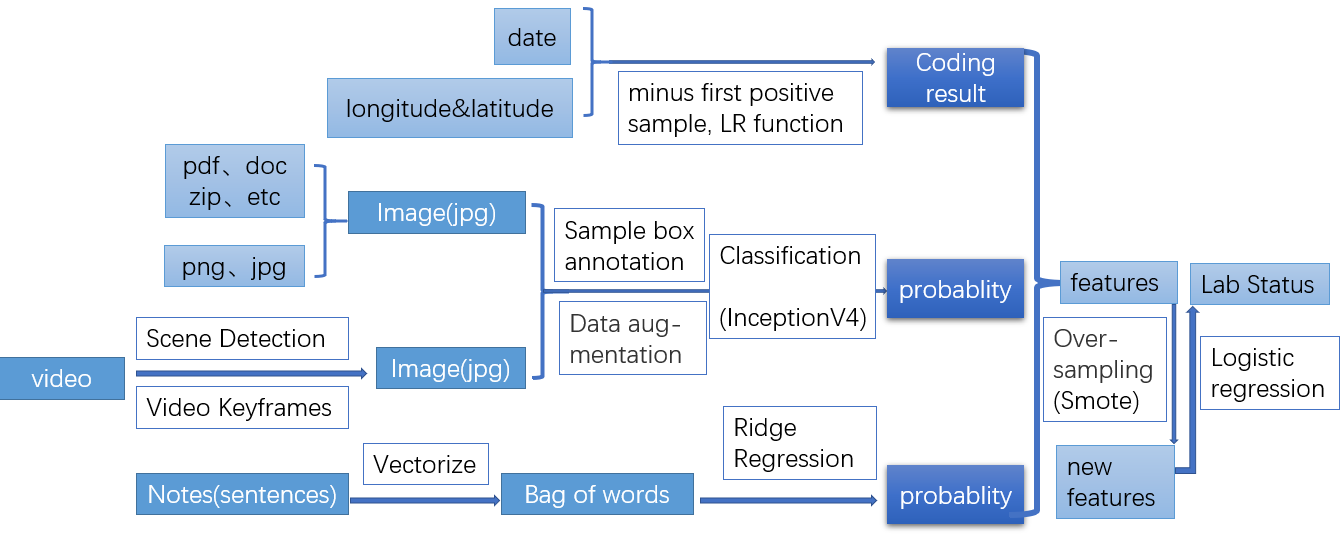
\includegraphics[width=18cm,height=8cm]{./pictures/problem2.png}\label{overall}
	\caption{Multimodal Classification Model}
\end{figure}


\subsection{Date, Longitude and Latitude Coding}
To deal with these three index, we do two steps:
\begin{enumerate}
	\item choose the first positive sample as reference(for date we counts the days between two samples) to eminate the influence of magnitude.
	\item \textbf{ LR function} for date, longitude and latitude:$f(x)=e^{-x}$.
	
\end{enumerate} 

The LR function can limit the number of these indexes in 0-1. And when new data comes in, the previous number don't have to change (compared with typical standardized).
\subsection{Video Processing}
In the given reports there are 92 vedio. Some videos almost keep quiet and can get quite clear image of the object, while others may contains great movement and can not recognize things clearly. In order to use all these information completely, we use \textbf{Scene Detection}to recognize \textbf{Scene Boundaries} and get\textbf{Video Keyframes} from video and porcess them with images together.

\subsubsection{Scene Detection}
Video scene detection algorithms generally use the degree of similarity difference between frames to measure, if the video frame is greater than a certain threshold, it is considered a new scene, otherwise it is not a new scene.

To do this there are mainly two ways:
\begin{itemize}
	\item \textbf{scikit-video}\cite{scikitvideo}:it uses the similarity between color and fringe to detect.
	\item \textbf{ffmpeg}\cite{ffmpeg}:it chooses the frames considering the compression degree.
\end{itemize}
Compared these two methods we use ffmpeg for it's quicker and moere efficient.

\subsubsection{Video Keyframes}
Video Keyframes are frames used for Video compression and Video codec and contain complete information. Other non-key frames will be compressed by the difference between them. Video frames can be divided into I,B,P three types.

And we firstly use \textbf{ffprobe} to get IBP frames, and than combine them to construct jpg image.
\fbox{%
	\parbox{\textwidth}{%
		
	\emph{\#ues ffprobe get IPB time:\\
			ffprobe -i 666051400.mp4 -v quiet -select\_streams v -show\_entries frame=pkt\_pts\_time,pict\_type \\
	\#transform IPB to jpg:\\
			ffmpeg -i 666051400.mp4 -vf "select=eq(pict\_type\,I)"  -vsync vfr -qscale:v 2 -f image2 ./\%08d.jpg}
	
	}%
}



\subsection{Image Processing}
After combine the image provided and the image produced from the video, we cope with them in two ways:
\begin{enumerate}
	\item \textbf{Sample box annotation} 
	\item \textbf{Data augmentation}
\end{enumerate}
to make the information for efficient thus improve classification's accuracy.


\subsubsection{Sample Box Annotation}
In many pictures, the insect is hidden in the environment such as flowers and woods and the size of the insect is small.

So it's hard to distinguish the insect through these pictures.To deal with these we try to annotate the object box .For the amount of pictures is large, we do this by  \textbf{YoloV5}\cite{Yolo}, an auto-annotate algorithm:
\begin{itemize}
	\item  First we annotate the sample box by hand to get 750 picture as trian data.
	\item  Then we use YoloV5 to deal with more than 2000 pictures.
\end{itemize}
The annotation result is pretty good as we can see in the picture below.

And as we can see in \ref{box}, the sizes of sample boxes are not uniform, so it's neccessary to do \textbf{Sample Box Annotation} to extract information correcetly.

\begin{figure}[H]
	\small
	\centering
	\begin{minipage}{5cm}
		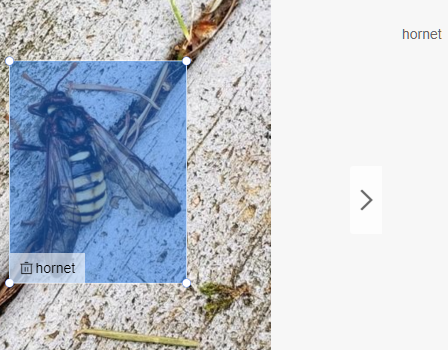
\includegraphics[width=5cm,height=5cm]{./pictures/hand1.png}
		\label{nt}
	\end{minipage}
	\begin{minipage}{5cm}
		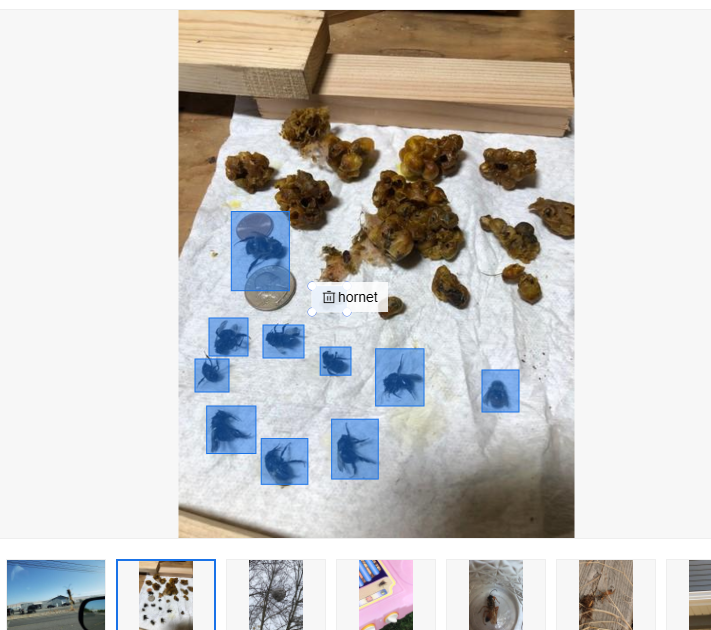
\includegraphics[width=5cm,height=5cm]{./pictures/head2.png}
		\label{nt}
	\end{minipage}
	\begin{minipage}{5cm}
		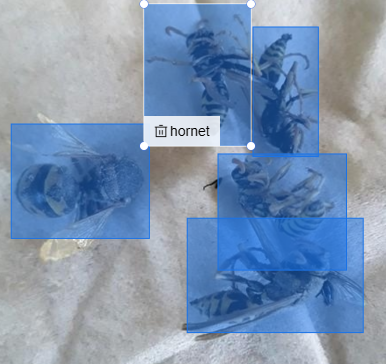
\includegraphics[width=5cm,height=5cm]{./pictures/head3.png}
		\label{nt}
	\end{minipage}
	\caption{Sample box annotation by hand}
\end{figure}

\begin{figure}[H]
	\small
	\centering
	\begin{minipage}{7cm}
		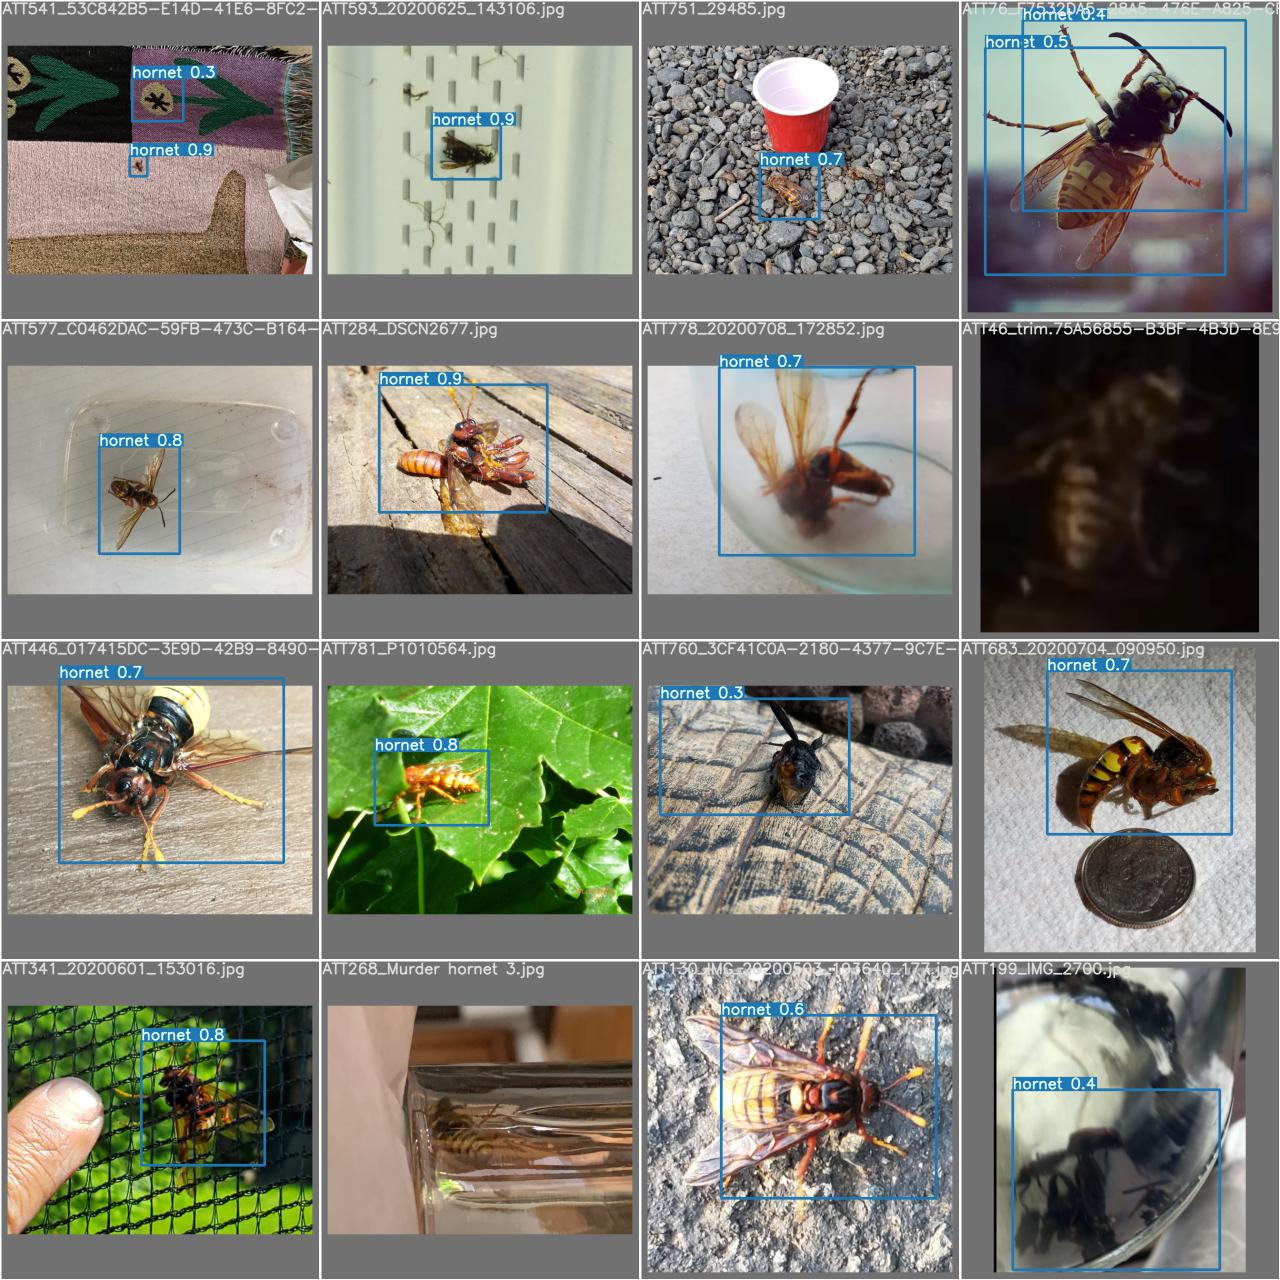
\includegraphics[width=7cm,height=6cm]{./pictures/machine1.png}
		\caption{Sample box annotation by yolo}\label{nt}
	\end{minipage}
	\begin{minipage}{7cm}
		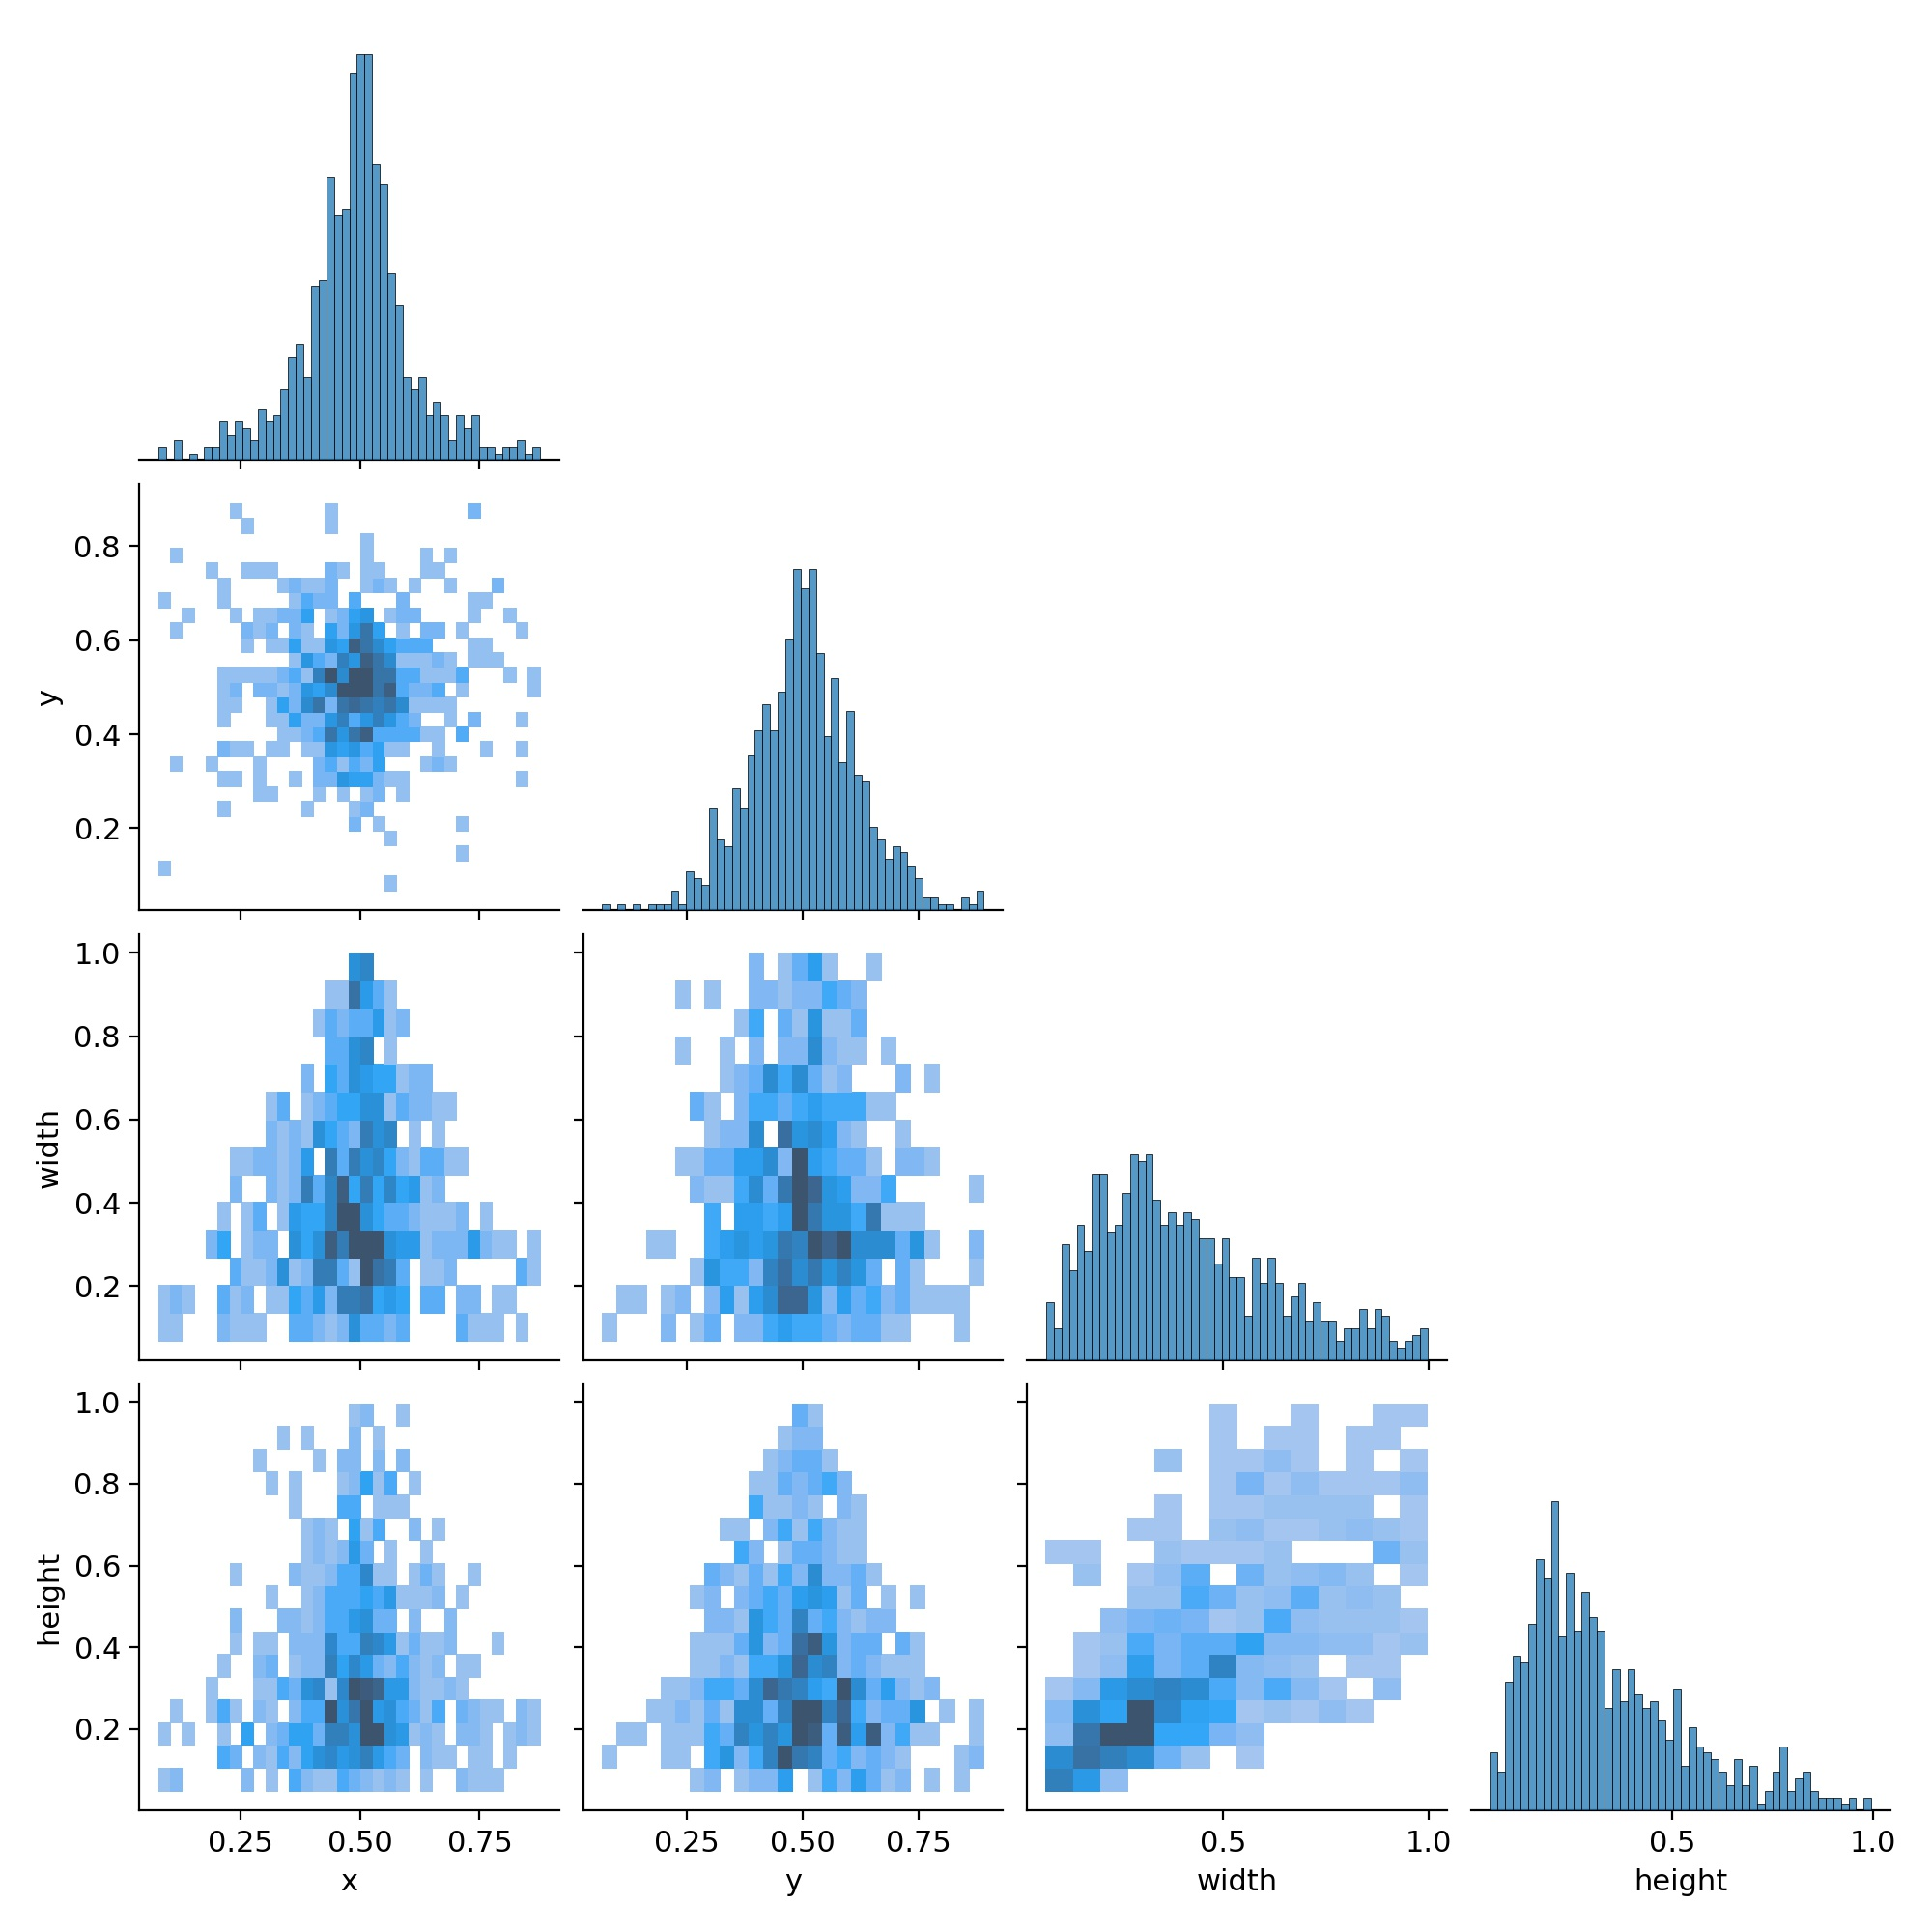
\includegraphics[width=7cm,height=6cm]{./pictures/picture_correlogram.png}
		\caption{the size and position of object boxs\protect\footnotemark[1]}
		\label{box}
	\end{minipage}
\end{figure}



\footnotetext[1]{x, y reprsent middle point of the object box,width and hight describe the shape. }

\subsubsection{Data Augmentation}
For the number of positive sample is too small, we use \textbf{data augmentation} to create more pictures from one positive sample through photo change. Thus we can get more information about how Asian Giant Hornet looks like.

As \ref{box} shows, the size and shape of the object box is not regular(The center of the sample frame is normally distributed and the height and width are skewed), so we choose to do the change randomly, that's to say the angle we rotate or the size we cut and other parameter are choosen randomly, so we can get more useful information.

Through this, we augment the positive sample(combined with the pictures provided by WSDA 26) 20 times and get 520 pictures.

More detailed operation can be seen in the table\ref{augm}, and a result can be seen in the picture\ref{augres}.

\begin{table}[H]
	\caption{Data augmentation operation}  \label{augm}
	\small
	\begin{center}  
		\begin{tabular}{|p{2cm}<{\centering}|p{14cm}|}  
			\hline  
			Operation &   python code\footnotemark[2]\\ \hline  
			Flip& RandomHorizontalFlip(),
			RandomVerticalFlip()\\ \hline  
			Rotation &RandomRotation(180, expand=True),
			RandomRotation(180, expand=False),\\  
			\hline 
			Affine& andomAffine(180, (0.3, 0.3), (0.4, 1), 3) \\  
			\hline  
			   Crop&RandomResizedCrop(size), 
			   transforms.RandomCrop(size, pad\_if\_needed=True),
			   transforms.CenterCrop(size),
			   transforms.RandomPerspective(distortion\_scale=0.3) \\  
			\hline
			 Color &  transforms.RandomGrayscale(0.2),
			 transforms.GaussianBlur(9),
			 transforms.ColorJitter(0.8, 0.8, 0.8, 0.4)\\  
			\hline
	
		\end{tabular}  
	\end{center}  
\end{table}
\footnotetext[2]{Python code using torchvision.transforms package. }


\begin{figure}[H]
	\small
	\centering
	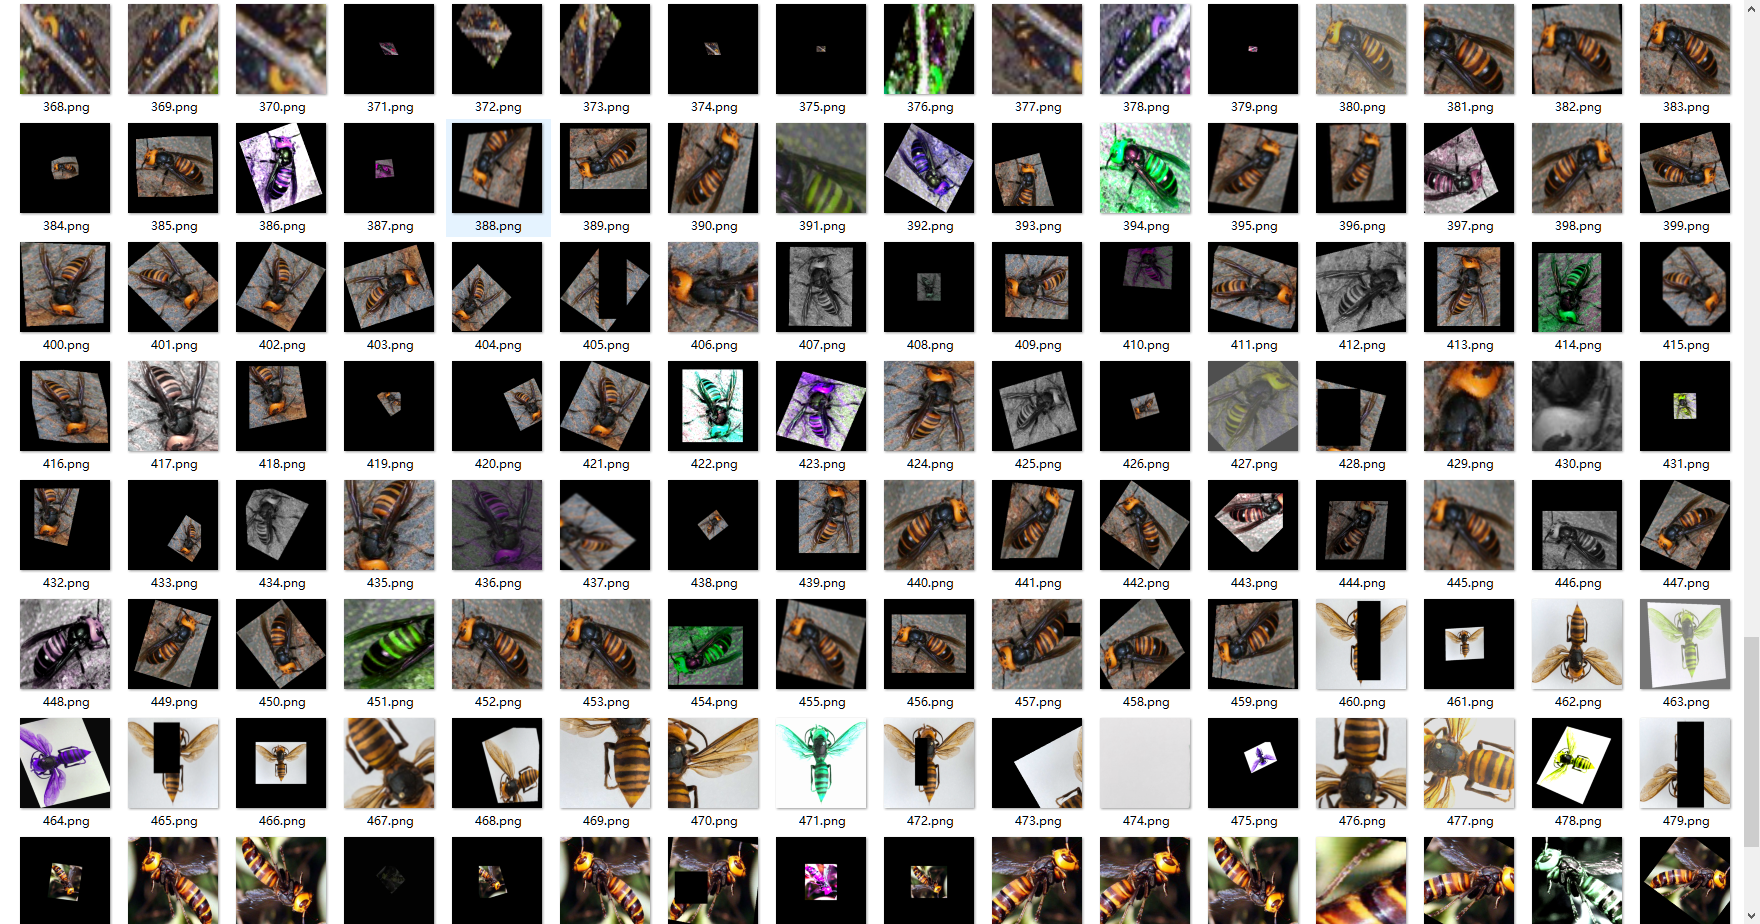
\includegraphics[width=14cm,height=6cm]{./pictures/angres.png}
	\caption{Some data augmentation result}\label{augres}
\end{figure}


\subsection{Image Feature Extraction}
\subsubsection{Algorithm:Inception V4}
After we process all the image and video, we get dozens of pictures. Then we need to extract features from these samples for further classification.

To do this, we choose a \textbf{CNN model} by GoogLeNet: \textbf{Inception V4}. For it is a typical model of image classification with many 1 dimension kernels which make it spends less time and space. And it is the \textbf{SOTA(state-of-the-art) model} in this area.
Following is the structure:\\
\textbf{Input--> Stem-->4$\times$ Inception A-->Reduction-A-->7$\times$ Inception-B-->Reduction-B--> 3$\times$Inception-C-->Average Pooling-->Dropout-->Softmax}

The end of the structure is a softmax layer, in these layer we can get the probability of being a hornet. And we use the probability as a feature.


\subsubsection{Loss Function:Focal Loss}
To deal with the imbalance of sample and make the positive sample easier to be detected, we use \textbf{focal loss} in Inception model \textbf{instead of cross entropy} to give more weight on the loss of small sample loss. Thus the postive model can be distinguished better.	
\begin{equation}
Focal\,Loss=-\alpha(1-p)^\gamma log(p)
\end{equation} 
\begin{center}
	p is the probability produced by the net, $\gamma=2,\alpha=0.25,0.75$
\end{center}

\subsubsection{K-folds}
For the lack of positive sample in trianing data may lead to great loss in model. We use \textbf{k-folds} to deal with the problem:
\begin{enumerate}
	\item Combine all the images and the augmented image together and shuffle them.
	\item Use 5-folds: every time choose $\frac{4}{5}$ of the data to train the model and leave the other $\frac{1}{5}$ for test.
	\item Choose the maxium of the loss as total loss, considering one sample may have many images(like video sample), some image is powerful while others maybe not be useful, so we should rely on the most powerful image to classify the sample.
	\item After parameter adjust, we use all the positive and negative data to\textbf{ retrain} the model.
\end{enumerate}


\subsection{Text Processing}
In the given infomation, there are notes and comments with each record,to deal with the words we need to code them first.We use \textbf{N-grams} to \textbf{vectorize} the sentence. This takes two steps:
\begin{enumerate}
	\item take adjacent words to construct combinations.
	\item represent the combinations with their frequency in whole sample.
\end{enumerate}

Through then we change a sentence into a string of numbers.
\begin{center}
	Example: 'One dead wasp seen in Blaine, and suspect flying nearby'\\
	$\Rightarrow$ [0 1 2 ... 0 0 0], dimension is 3000
\end{center}
\subsection{Text Feature Extraction}
After coding the notes, we use \textbf{ridge classification} to classify the notes and get the probability of a sample being a hornet. Ridge classification add penalty term to ordinary model, thus the effect of \textbf{multicollinearity} due to the high dimension can be eliminate.
\begin{equation*}
x=[x_1,x_2,....,x_{3000}], \qquad y=1(positive)\,or\,0(negative)
\end{equation*}
\begin{equation}
y=\sum_{i=1}^{3000} \beta_i x_i+\beta_0
\end{equation}
\begin{equation}
\beta^{ridge}=argmin_{\beta}\lbrace \sum_{i=1}^{N}(y_i-\beta_0-\sum_{j=1}^{3000}\beta_j x_j)^2+\lambda\sum_{i=1}^{3000}\beta_j^2,\qquad N:sample\,size
\end{equation}

\subsection{Overall Classification}
\subsubsection{Feature Combination}
We combine all the features below to be a 5 dimensional vector as \textbf{independent variable}
\begin{center}
X=[longitude coding,latitude coding,date coding,image probability,\\language probability,if sample has photo/video]
\end{center}

And use "Lab Status": Y=1 (if Postive),0(if Negative) as \textbf{dependent variable}



\subsubsection{Smote}
\begin{figure}[H]
	\small
	\label{u=tsne}
	\centering
	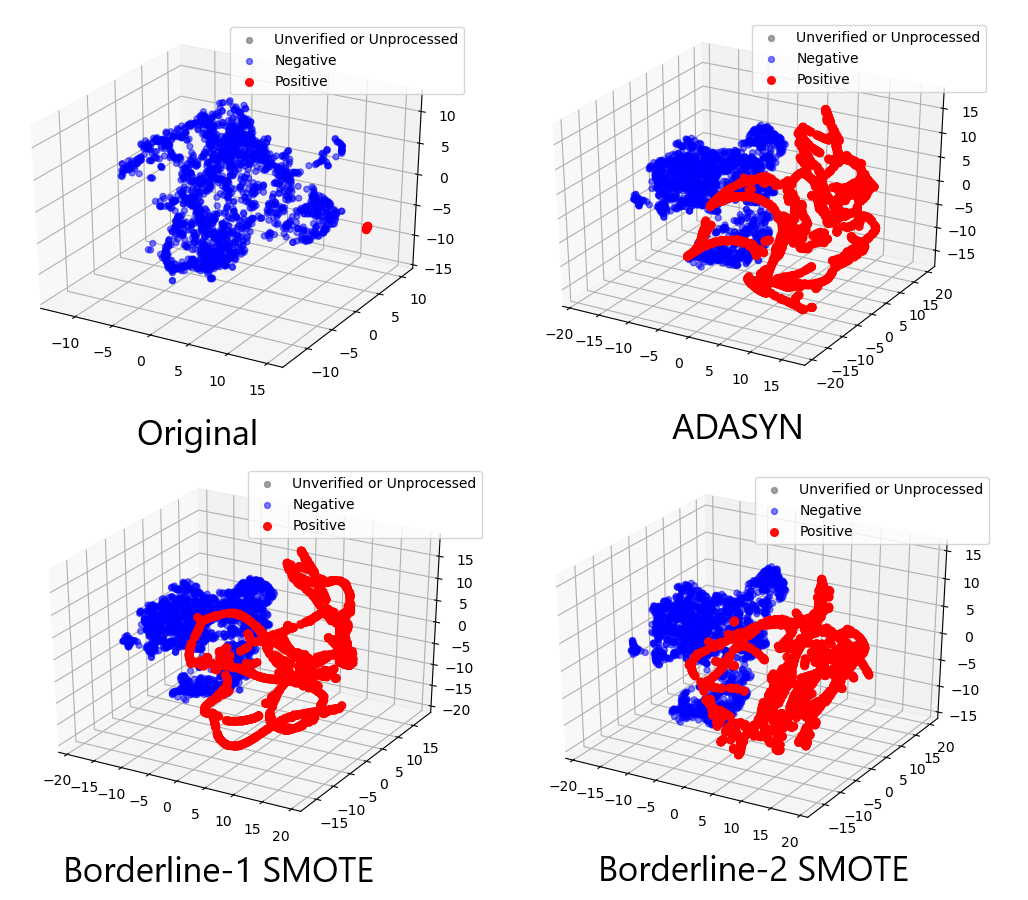
\includegraphics[width=13cm,height=11cm]{./pictures/tsne.png}
	\caption{t-SNE T-Distributed of Original Sample and Samples through Three Over-Sampling Method}\protect\footnotemark[1] 
\end{figure}
\footnotetext[1]{ t-SNE \cite{Smote} is a tool to visualize high-dimensional data. It converts similarities between data points to joint probabilities and tries to minimize the Kullback-Leibler divergence between the joint probabilities of the low-dimensional embedding and the high-dimensional data. We use PCA result as the original number and iterate 500 times.}

As is shown in Figure\protect\ref{u=tsne},all these features satisfied \textbf{Manifold assumption} so the classification is reasonal and the features are usable.

The only problem is that the positive samples are too scarce, so we need to over-sample them. The most intuitive method is randomly repeat those positive samples with techniques like Bootstrap and this will not change the space distribution of them, but actually they are too concentrated on one point and our classifier may lay down the border anywhere between two clusters, which is not desired. What's more, slight noices will prevent over-fitting and help increase the robustness of our model.

we introduce SMOTE(Synthetic Minority Oversampling Technique)\cite{Smote1} and \textbf{ADASYN}(Adaptive Synthetic Sampling)for over-sampling for we want more noise to train the model. It focuses on generating minority class sample near the border of the minority class and majority class. In this problem, it can strengthen the border near positive and negative samples.


SMOTE algorithm contains three steps:
\begin{enumerate}
	\item For everyone in the positive sample, get its k-neighbor positive points(by Euclidean distance )
	\item Choose sampling ratio n. For each positive sample x, selected n points from the k points in the first step for $x_k,k=1,2,...,n$. 
	\item: For each $x_n$, create new point: $x_{new}=x+\epsilon(x-x_n), where \epsilon \sim U(0,1)$
\end{enumerate}

Then, we get new points added to our samples. ADASYN is an improvised algorithm based on SMOTE. More details of this method are accessible in \cite{Smote3}

\subsubsection{Logistic Regression}
We conduct \textbf{logistic regression} to evaluate all the features and set up a model to classify the records. And the model of logistic regression is showed below:

\begin{equation}
y=\frac{1}{1+e^{-z}},\qquad z=\omega^Tx+b 
\end{equation}
\begin{center}
	$\omega,b:parameter,\qquad y:the\, probability\, to \,be\, positive$
\end{center}

\section{Task 3: Classify Unverified Reports}
Using the model in problem 2, we conduct the same process to calculate the features and take all the verified reports as the training dataset to fit the two-stage model. We use the model to \textbf{predict the probabilty of the unverified points to be positive}. Output of each stage can be adjusted to a fraction between 0 and 1, indicating the likelihood of the current predicting report is an Asian Giant Hornet sighting. 
\subsection{Predict Result}

\begin{figure}[H]
	\small
	\centering
	\begin{minipage}{5cm}
		\label{prob}
		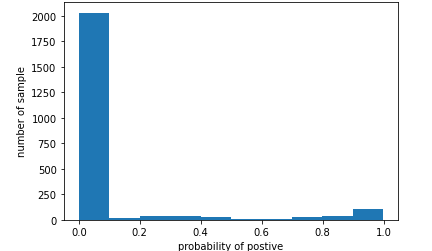
\includegraphics[width=5cm,height=4cm]{./pictures/prob.png}
		\caption{The distribution of positive probability of unverified sample} 
	\end{minipage}
	\begin{minipage}{4cm}
		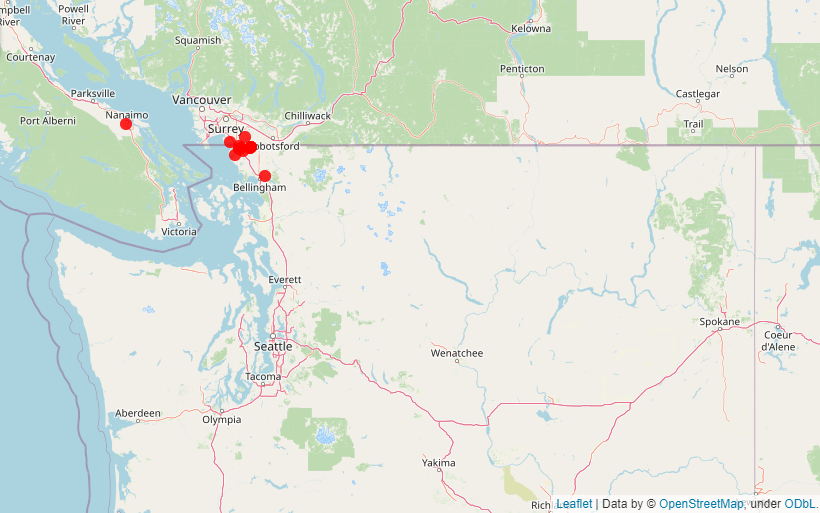
\includegraphics[width=4cm,height=4cm]{./pictures/pos.png}
		\caption{Distribute of original positive samples}
	\end{minipage}
	\begin{minipage}{4cm}
		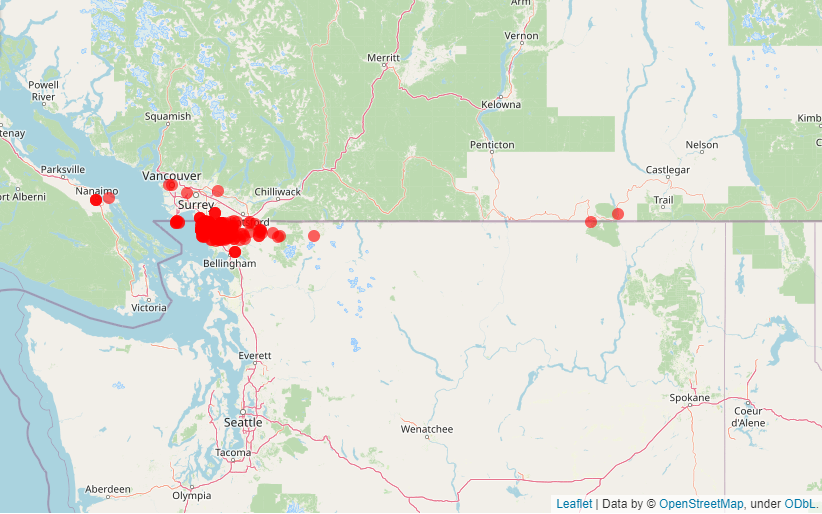
\includegraphics[width=4cm,height=4cm]{./pictures/addun.png}
		\caption{Positive samples and unverified with probability>0.75}
	\end{minipage}
\end{figure}
Figure \ref{prob} has shown the probability we get through the model in task two.And the other two pictures show the distribution of positive sample after add the unverified sample whose has more than 0.75 probability to be positive.


\section{Task 4: Model Update}
Considering the model is complex and the training data is huge, it would spend great long time and quite large space to retrain the model. So when construct the model when have considered this problem to guarantee \textbf{online learning},that means we can update our model given a new sample in a quite short time. So \textbf{we can tune the model as soon as new sample comes in}.

The adjustment of model can be divided into two parts:
\begin{itemize}
	\item \textbf{Feature Engineering Part} :process new sample
	\item \textbf{Model Fine-Tuning Part} :adjuest the parameters in learning model.
\end{itemize}
\subsection{Feature Engineering Part}
\begin{itemize}
	\item \textbf{Longitude ,Latitude and Date}:For these three index we only need to do: $\hat{x}=e^{-(x-x_{1^{st}positive})},x=longitude/latitude/date$. Then, we can get coding result.
	\item \textbf{Video and Image}: For video,we only need to do the same: scene detection and video keyframes to transfer a video into some images. Then, for
	\item \textbf{Yolo} has trained well and can get object box automatically, and when the "Lab Status" is postive, it will be augmented as well.
	\item \textbf{Text}To deal with the notes,when we do \textbf{n-grams}, we have set up dictionary to the coding to the most frequent 3000 words and phrases. So when new sentence comes in, we only need to code the sentence by the coding dictionary.
\end{itemize}


\subsection{Model Fine-Tuning Part}
In this part, we adjust the parameter of the model as new sample comes in,and we need to make sure the model is \textbf{robust, time-saving, space-saving},thus it can update on time.

Considering all these we use \textbf{FTRL} and \textbf{Fine-Tune} to do this part.
 
\subsubsection{Fine-Tune}
There are mainly three classification model in the overall process:
\begin{itemize}
	\item Ridge Classification for language coding
	\item Inception V4 for image
	\item Logistic Regression for all features
\end{itemize}

Between these Inception V4 is much more complicated and spends much more time to train.  So for this part, we choose to keep most of the net fixed and just adjust weights of the end of the net: softmax layer. So the \textbf{fine-tune} would make the result easier to converge and save more time.

\subsubsection{Online optimizer: FTRL}
\begin{table}[H]
	\begin{center}
		\caption{Notations}
		\begin{tabular}{cl}
			\toprule
			\multicolumn{1}{m{3cm}}{\centering Symbol}
			&\multicolumn{1}{m{8cm}}{\centering Definition}\\
			\midrule
			$T$& Total iterationround\\
			$t$& The round of iteration \\
			$l$&Loss function\\
			$w$&Parameters\\
			$W$&The range of parameters\\
			$g$& The gradient of losss function by parameters\\
			$\eta$&Learning rate\\
			$\lambda_1$&Regularization coefficient\\
			\bottomrule
		\end{tabular}\label{Ntt}
	\end{center}
\end{table}
To deal with the robust of model tuning and optimize the model as we have new report, we choose \textbf{FTRL}  algorithm and pack it as an optimizer.

And use it in updating ridge classification, Inception V4 and logistic regression.

For this model can decrease regret($Regret=\sum_{t=1}^T l_t(w_t)-min_{W}\sum_{t=1}^Tl_t(w)$)and increase sparsity. So  we take less space and the model is more accurate. Here is the iterate formula.



\begin{equation}\mathbf{w}_{t+1} = \underset{\rm \mathbf{w}}{\rm arg\ min}\left(\displaystyle\sum_{s=1}^t {\mathbf{g}_s \cdot \mathbf{w}} + \frac 12 \displaystyle\sum_{s=1}^t {\sigma_s||\mathbf{w} - \mathbf{w}_s||_2^2} + \lambda_1||\mathbf{w}||_1\right),\qquad \sum_{s=1}^t \sigma_s = \frac 1{\eta_t}\end{equation}

\subsubsection{Updating Process}
After we treat the new report as feature engineering part shows, we send these data to tuning these model and save the model as \ref{overall} shows. And repeat this once a new report comes.



\section{Task 5: Hornet in Washington State}



\section{Model Evaluation and Testing}
\subsection{Ablation Experiment for Focal Loss }
To test whether focal loss is efficient, we do an \textbf{Ablation Experiemt }as below:
\subsubsection{Model}
\begin{equation*}
The\,accuracy\,of\,model:y=\mu+\epsilon,\qquad \epsilon\sim N(0,\sigma^2)
\end{equation*}
\textbf{Hypothesis}:Image classification is more efficient by focal loss instead of BCE(Binary Cross Entropy)
\begin{equation*}
H1:\mu_1<\mu2\leftrightarrow H2:\mu_1\geq \mu_2
\end{equation*}
$y_1=\mu_1+\epsilon_1,y_2=\mu_2+\epsilon_2$,$y_1,y_2$represent the accuracy by focal loss and BCE respectively.

We use \textbf{T test} to verify the hypothesis.
\subsubsection{Test}
As we use 5-fold method to go through the model, so we can get 5 samples in each case:$y_{11},y_{12},y_{13},y_{14},y_{15}$ and $y_{21},y_{22},y_{23},y_{24},y_{25}$.

By using the two strings data to do T-test, And find out that focal loss is efficient when \textbf{significance is 0.1}.



\section{Strengths, Weaknesses and Improved Method}
\subsection{Strengths}
\textbf{Strength 1}: The classification model is a two-stage, using separate networks for different features in multimodal data sets. So:
\begin{itemize}
	\item  It is flexiable and transferable, (Like object box annotation and image calssification, we can change another model and guarantee the result is end to end as well), also if we use independent outside dataset, like the AGH dataset from Biology Department or introduce industrial-grade model such as GPT in NLP area to handle notes, the model also works.
	\item  The model is decoupling, so when the image or the text is missing, it can still do classification. So the model is quite robust.
\end{itemize}

\textbf{Strength 2}: The classification model is an online learning model. Once a new sample comes, the model can be updated quickly. So this great improves time and space efficiency and let the model constantly optimizable.

\subsection{Weaknesses}
\textbf{Weakness 1:}The testing for the first task is not enough,we just consider the tend of the center of whole the hornet,but ignore the situation for each colony.

\subsection{Improved Method}
\textbf{Take the environment of image into consideration}
In image classification part, we didn't consider the environment(like cave or hornet nest,etc). The attachment of the problem introduces that the nest of Asian Gaint Hornet is special, and they live in the area near the ground and don't like to go around the flowers as well.So we may excavate this with more background information.

\clearpage
\section*{Memo}\addcontentsline{toc}{section}{Memo}
	\begin{flushleft}
		Dear Governors,
	\end{flushleft}
	
	We are writing to inform you our achievement after performing data analysis and modeling. Based on the data provided by the public reports, we have developed a data-driven framework that can be used for both prediction and inference and update its model given new reports over time.

	Our framework are structured as follows, which can be used for identifying this pest when new data comes in.
	\begin{enumerate}[\bf 1.]
		\item \textbf{Converting different kinds of data }
		
		We adopted a series of method to handle different types of data:
		
		video:\\
		Use the Scene Detection and Video Keyframes to transform the video into images, and use these images for future analysis.\\
		Image:\\
		First use Sample box annotation and Data augmentation to use the information of images more efficiently. Use trained CNN model Inception V4 with online learning method FTRL and Fine-Tune to update the model and calculate the the probability of being a hornet for new data (image score).
		text:\\
		When new data come in, use N-grams to vectorize the sentence and calculate the frequencies of 3000 feature words. Then based on the ridge regression model trained above, we use online learning method FTRL and Fine-Tune to update the model, and get the probability of being a hornet for new data (text score).
		\item \textbf{Performing the penalized logistic regression model}
		You have got the text score, image score and some other features of the new sample from above, now use the trained the penalized logistic regression model combined with online learning method FTRL and Fine-Tune to update the model, and get the resulting probability.
	\end{enumerate}
	Some highlights of our framework:
	
	\begin{enumerate}[\bf 1.]
		\item \textbf{Strategies to deal with imbalanced data}
		We found that labelled data are classified into two imbalanced categories (Positive ID: 14, Negative ID: 2096) based on a brief observation of the data. Imbalanced data will make the model tend to classify new data into the Negative since it can result higher accuracy. In that case, the model is possibly incorrect. To handle this problem, we adopt a series of methods:\\
		(1) Use focal loss to make positive sample easier to be detected.\\
		(2) Use Synthetic Minority Oversampling Technique (SMOTE) to create artificial positive sample in logistic regression model.
		\item \textbf{Online learning methods}
		We use online learning method FTRL and Fine-Tune to update the model when new data comes in, reduce the computation time and make quick classificaiton.
		
		
		Moreover, this data-driven framework can be extended to other similar problem, especially those problem with multitype data. You can adopt the framework deal with and train specific model to detect other pests in Washington State. Also, the SMOTE method implemented in the framework can deal with more general classification problem with imbalanced data.
	\end{enumerate}
		
\clearpage
\begin{thebibliography}{99}
	\addcontentsline{toc}{section}{References}  %引用部分标题("Refenrence")的重命名
	\bibitem{fb}Facebook.Asian Giant Hornet Watch.https://www.facebook.com/groups/hornets.
	\bibitem{website}Washington State Department of Agriculture. 2020 Asian Giant Hornet Public 
	Dashboard. https://agr.wa.gov/departments/insects-pests-and-weeds/insects/hornets/data.
	\bibitem{wiki}Wikipedia.Asian Giant Hornet. https://en.wikipedia.org/wiki/Asian\_giant\_hornet.
	\bibitem{scikitvideo}Scikit-Video .https://github.com/scikit-video/scikit-video/blob/master/skvideo/measure/scene.py.
	\bibitem{ffmpeg}ffmpeg . https://ffmpeg.org/ffmpeg-filters.html\#select\_002c-aselect.
	\bibitem{Yolo}YoloV5 . https://github.com/topics/yolov5
	\bibitem{Smote}van der Maaten, L.J.P.; Hinton, G.E. Visualizing High-Dimensional Data Using t-SNE. Journal of Machine Learning Research 9:2579-2605, 2008.
	\bibitem{Smote1}Haibo He, Yang Bai, Edwardo A Garcia, and Shutao Li. Adasyn: adaptive synthetic sampling approach for imbalanced learning. In 2008 IEEE International Joint Conference on Neural Networks (IEEE World Congress on Computational Intelligence), 1322–1328. IEEE, 2008.
	\bibitem{Smote3}N. V. Chawla, K. W. Bowyer, L. O.Hall, W. P. Kegelmeyer, “SMOTE: synthetic minority over-sampling technique,” Journal of artificial intelligence research, 321-357, 2002.
\end{thebibliography}

\clearpage

\section*{Appendices}\addcontentsline{toc}{section}{Appendices}
	\noindent Appendix1:
	%下面的是配置是可以写中文注释的python环境:
	%\usepackage{listings}
	%\usepackage{color}
	\definecolor{dkgreen}{rgb}{0,0.6,0}
	\definecolor{gray}{rgb}{0.5,0.5,0.5}
	\definecolor{mauve}{rgb}{0.58,0,0.82}
	\lstset{	frame=shadowbox,                           % shadowbox framed
		rulesepcolor= \color{gray},%框的颜色
		language=Python,
		aboveskip=3mm,
		belowskip=3mm,
		showstringspaces=false,
		columns=flexible,
		basicstyle={\small\ttfamily},
		numbers=left,%设置行号位置none不显示行号
		%numberstyle=\tiny\courier, %设置行号大小  
		numberstyle=\tiny\color{gray},
		keywordstyle=\color{blue},
		commentstyle=\color{dkgreen},
		stringstyle=\color{mauve},
		breaklines=true,
		breakatwhitespace=true,
		escapeinside=``,%逃逸字符(1左面的键),用于显示中文例如在代码中`中文...`
		tabsize=4,
		extendedchars=false %解决代码跨页时,章节标题,页眉等汉字不显示的问题  
	}
	\begin{lstlisting}
	
	\end{lstlisting}
	
	

%%%%%%%%%%%%%%%%%%%%%%%%%%%%%%
\end{document}
